\chapter{Evaluation}
\label{chapt:evaluation}

This chapter describes the evaluation of the two different implementation of the system architecture. (1) By introducing more than one memcached instances at layer 2 as figure \ref{fig:system_architecture} shows and (2) by introducing more than one Social Network engines at layer 1.

\section{Improving Performance with memcached}
\label{sec:eval_memcache}  
The test perform with the following loads: (L1) ten users requests two applications consecutively one hundred times, (L2) ten users requests four applications consecutively one hundred times and (L3) ten users requests eight applications consecutively one hundred times. In this experiment we kept constant the following components of system: the Elgg front-end apache server, the Social network database, and the CDO server - client communication. In the system, increased the number of memcached nodes.
The figure~\ref{fig:} shows the  average, minimum and maximum response time with the following system configuration: (C1) no memcached node, (C2) one memcache node added and (C3) two memcache nodes added.

\begin{figure}[h]
	\caption{The average response time for all configurations.}
	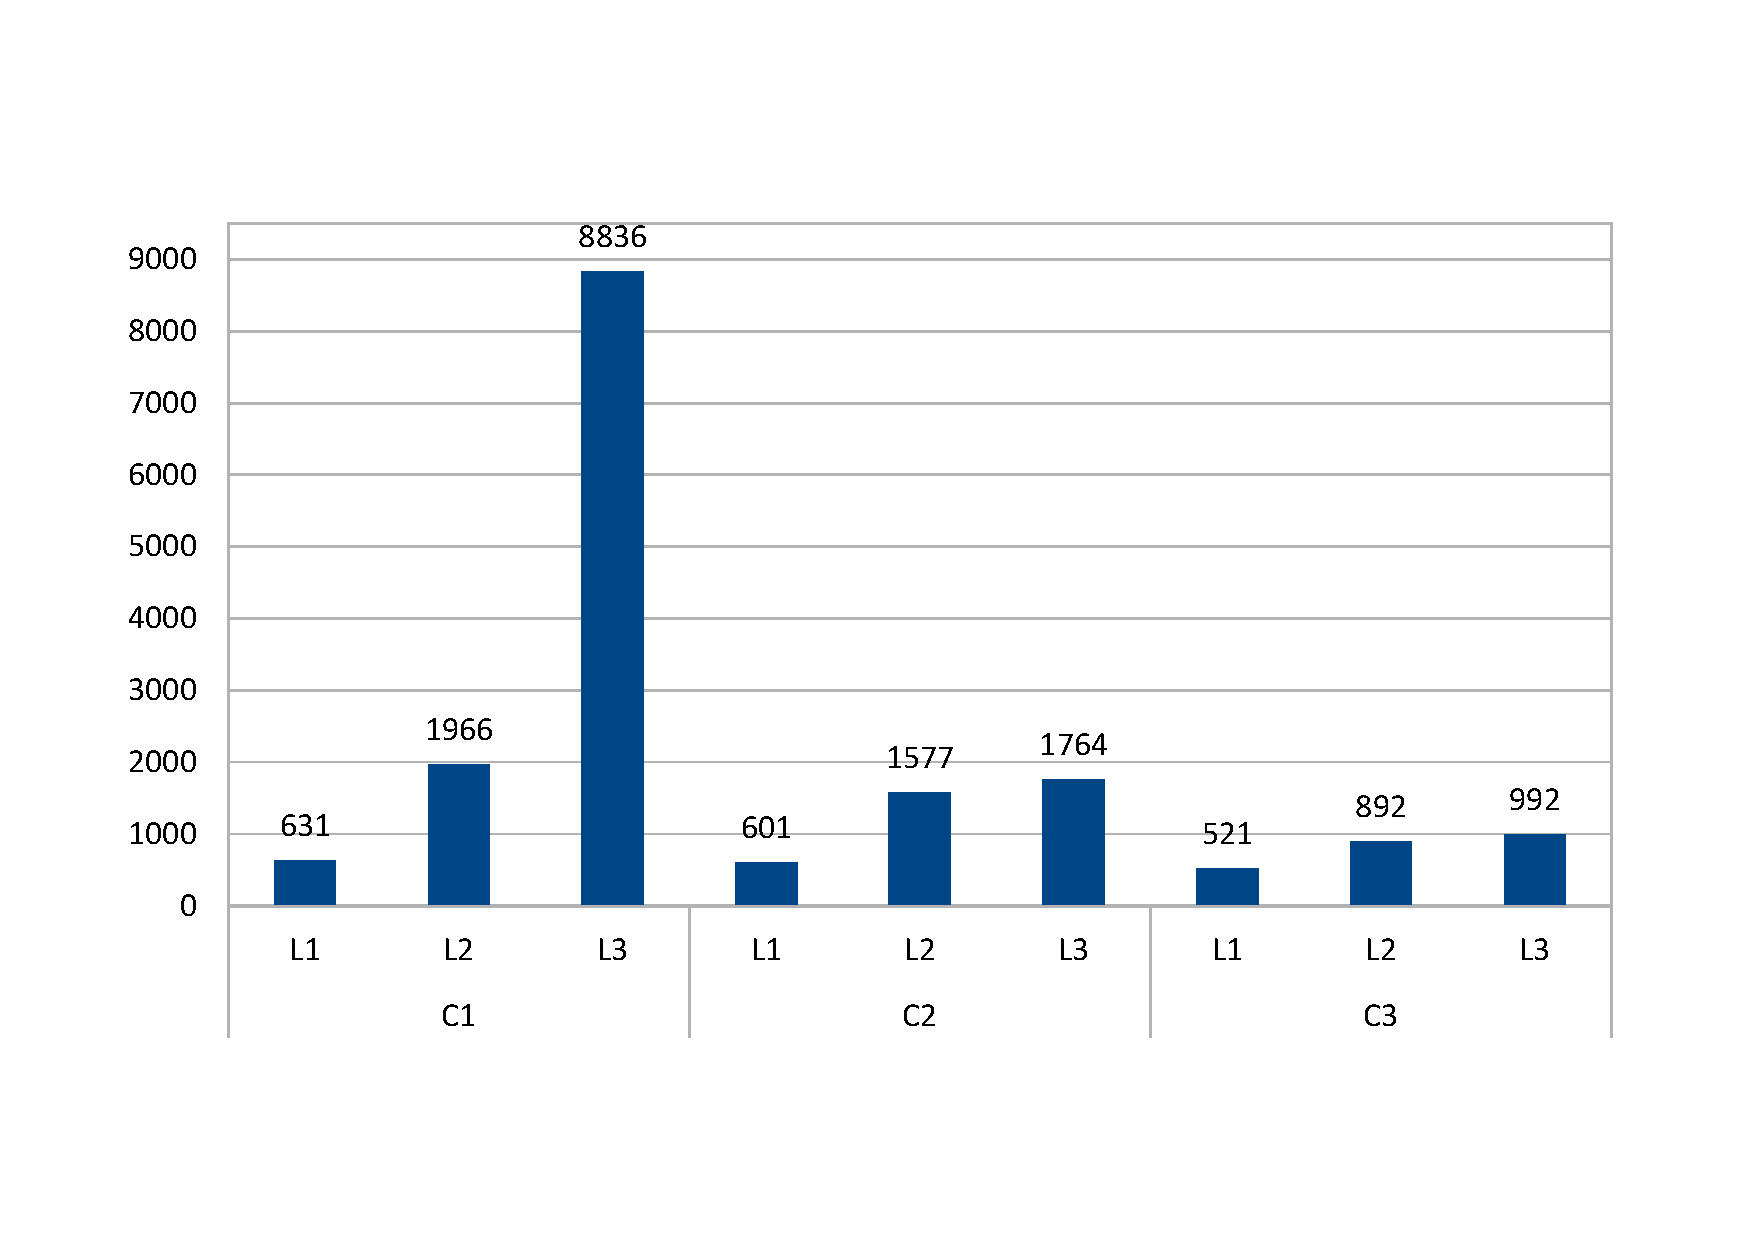
\includegraphics[width=0.6\textwidth,natwidth=200,natheight=150]{./fig/RTavg.pdf}
	\centering
	\label{fig:rtavg}
\end{figure}
\section{Improving Performance with engine}
